When creating test cases to check the validity of the transition function outlined in Section~\ref{sec:overview-delta} we broke down our test cases to exploit the different types of failures on the lattice. Our first constraint of the walk was to begin at (0,0). It is tested by the value of the start state, if the walk could pass this it would move out to check for jumps, branches and closure properties. A jump on the lattice can happen in one of two ways: horizontal or vertical. A branch can happen in one of many ways depending on what is a valid input from the next, the idea is that whatever node the state is currently in can only transfer to one or the other but not both. Closure properties test for self-avoiding walks, so we created test cases that would demonstrate the delta function knew how to proceed. We ran over 50 test cases through the DFA. In the following paragraphs, we present 4 examples of these and discuss the sequence of states that leads to acceptance or not.

\begin{figure}[h!]
\begin{center}
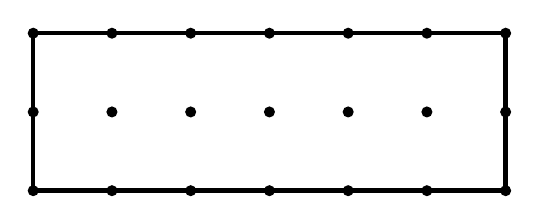
\begin{tikzpicture}
\foreach \x in {0,...,6}
\foreach \y in {0,1,2}
{
\fill (\x,\y) circle (2pt);
}

\draw [ultra thick] (0,0) -- (6,0) -- (6,2) -- (0,2) -- (0,0);

\end{tikzpicture}
\end{center}
\caption{Test case to illustrate branch identification and rejection.}
\label{fig:test-branch}
\end{figure}
The input in Figure~\ref{fig:test-branch} illustrates how a branch condition results in rejecting an invalid state. After the initial input is processed, for this to be a valid walk it must proceed from the top (walks must originate at the origin). After the next input is read this would transition to the dead state. Code to identify branches successfully detected that this input diverged into two paths. Once the DFA is in the dead state, we know the input is invalid.

\begin{figure}[h!]
\begin{center}
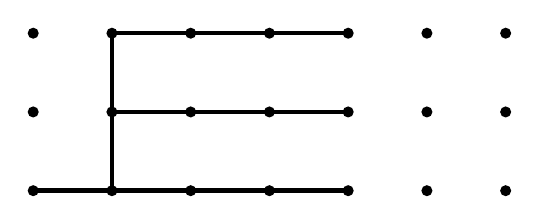
\begin{tikzpicture}
\foreach \x in {0,...,6}
\foreach \y in {0,1,2}
{
\fill (\x,\y) circle (2pt);
}

\draw [ultra thick] (0,0) -- (1,0) -- (2,0) -- (3,0) -- (4,0);
\draw [ultra thick] (1,0) -- (1,1) -- (1,2);
\draw [ultra thick] (1,1) -- (2,1) -- (3,1) -- (4,1);
\draw [ultra thick] (1,2) -- (2,2) -- (3,2) -- (4,2);

\end{tikzpicture}
\end{center}
\caption{Test case to illustrate multiple branch identification.}
\label{fig:mult-branch} 
\end{figure}
The input in Figure~\ref{fig:mult-branch} demonstrates the branch identification capabilities of the DFA. It is clear that there has been a branch after the third input symbol because several of the resulting vertices have degree 3. It is possible to transition to a triple-ended state from a single-ended one, but this example is not a valid way.

\begin{figure}[h!]
\begin{center}
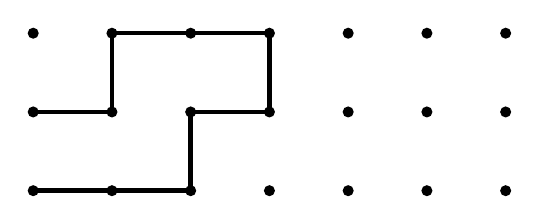
\begin{tikzpicture}
\foreach \x in {0,...,6}
\foreach \y in {0,1,2}
{
\fill (\x,\y) circle (2pt);
}

\draw [ultra thick] (0,0) -- (1,0) -- (2,0) -- (2,1) -- (3,1) -- (3,2) -- (2,2) -- (1,2) -- (1,1) -- (0,1);

\end{tikzpicture}
\end{center}
\caption{Test case to illustrate double-ended state resulting in a valid walk.}
\label{fig:double-ended}
\end{figure}
Execution of the DFA on the input presented in Figure~\ref{fig:double-ended} shows that once the DFA is in a double-ended state, it must remain in a double-ended state. The input continues in a double-ended state and is accepted upon being closed.

\begin{figure}[h!]
\begin{center}
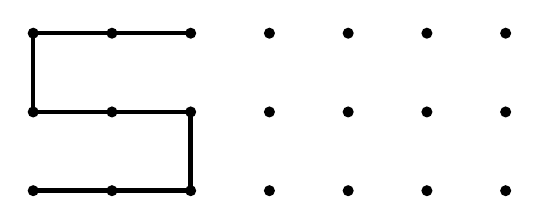
\begin{tikzpicture}
\foreach \x in {0,...,6}
\foreach \y in {0,1,2}
{
\fill (\x,\y) circle (2pt);
}

\draw [ultra thick] (0,0) -- (1,0) -- (2,0) -- (2,1) -- (1,1) -- (0,1) -- (0,2) -- (1,2) -- (2,2);

\end{tikzpicture}
\end{center}
\caption{Test case to illustrate triple-ended state behavior.}
\label{fig:triple-ended}
\end{figure}
The input in Figure~\ref{fig:triple-ended} begins in a triple-ended state. The third input closes two of the paths (recall that valid input from triple-ended state must connect all the nodes to proceed). After the final nontrivial input, the DFA is in a single-ended, accepting state.
